\documentclass{report}

\usepackage[shortlabels]{enumitem}
\usepackage{pgfplots}
\pgfplotsset{compat=1.18}

\input{preamble}
\input{macros}
\input{letterfonts}

\title{\Huge{Review over some Math} \\ \vspace{1cm} \normalsize{Notes on the book `All the Math You Missed But Need to Know for Graduate School' by Thomas A. Garrity}, \\ along with some personal thoughts and excercise solutions.}
\author{\huge{José Daniel Mejía C.}}
\date{2026}

\begin{document}

\maketitle
\newpage% or \cleardoublepage
% \pdfbookmark[<level>]{<title>}{<dest>}
\pdfbookmark[section]{\contentsname}{toc}
\tableofcontents
\pagebreak

\chapter{Summary over topics}
\section{Structure of mathematics}
\subsection{Equivalence problems}

Several problems or fields of study in math come down to seeing if two or more objects are the `same', or detecting their differences.

\nt{The concept of two objects being the same depends on the field of study.}


\textbf{Equivalence} between two objects can be explained by the allowed Maps or functions between them.

\ex{}{A square and a circle are equivalent in topology; they can be stretched out from one to the other.
\\
They are not the same in differential geometry; one is smooth (differentiable) and the other is not.}

\textbf{Invariants} are properties that two or more object must satisfy if they are equivalent, however they themselves do not determine equivalence between them.

\ex{}{In topology, two circles are not equivalent to a single circle. The two circles have two connected components, whereas the one only has one connected component. Hence, both objects are not equivalent.
\\
However, a sphere and a circle have the same number of connected components, but they are not equivalent.}

\subsection{Functions}
Functions describe all kinds of situations, both in the real world and in an abstract matter.

Each field of study or area in mathematics focuses in a specific kind of function. Calculus studies differentiable functions fron $\RR \to \RR$, for example.

\pagebreak

\section{Topics}

\subsection{Linear Algebra}
Linear algebra studies \textbf{Linear Transformations} and \textbf{Vector Spaces}. A linear transformation has a matrix representation, given a basis for the vector space being considered.

Two or more different matrices can represent the same transformation, but over different choices of bases of the same vector space.

The key theorem in linear algebra explains several equivalent descriptions for when a matrix, and hence the associated transformation, is invertible.

Other important aspect is understanding the occurrence and usefulness of eigenvectors and eigenvalues.

\subsection{Real Analysis}
The definitions of \textbf{Limit}, \textbf{Continuity}, \textbf{Differentiation} and \textbf{Integration} are given in terms of $\epsilon$ and $\delta$. \textbf{Uniform Convergence} of functions is a key part of this topic.

\subsection{Differentiating Vector-Valued Functions}
The \textbf{Inverse Function Theorem} explains that a differentiable function $f : \RR \to \RR^n$ is invertible iff the determinant of its derivative (the Jacobian) is never zero.

It is important to understand what it means for a vector-valued function to be differentiable, and why its derivative must always be a linear map, represented by the Jacobian as a matrix.

Understanding the \textbf{Implicit function theorem} and how it relates to the Inverse Function Theorem is also relevant.

\subsection{Point Set Topology}
The concept of \textbf{Open Sets} and how a \textbf{Topology} can be built in terms of open sets must be understood. Also how a function is said to be \textbf{Continuous} in terms of open sets is key.

The standard topology in $\RR^n$ and the \textbf{Heine-Borel Theorem} is covered, as well as what a metric space is and how a topology is defined using its metric.

\subsection{Classical Stokes' Theorem}
The calculus of vector fields covers the \textbf{Curl}, and \textbf{Divergence} of vector fields, the \textbf{Gradient} of a function and the \textbf{Path Integral} along a curve.

The \textbf{Divergence Theorem} and \textbf{Stokes' Theorem} are presented as classical extensions of the Fundamental Theorem of Calculus, it is relevant to understand why they are indeed extensions of this classic theorem.

\subsection{Differential Forms and Stokes' Theorem}
\textbf{Manifolds} are geometric objects. \textbf{Differential $k$-forms} allows calculus to be done on manifolds. There are several ways to define a manifold. How to think about and define differential $k$-forms, and how to take their \textbf{external derivative} is important.

Differential $k$-forms and external derivatives can be represented using vector fields, gradients, curls and divergences.

The statement of \textbf{Stokes' Theorem} in this context is covered, and special cases over the Divergence Theorem and Stokes' Theorem seen before.

\subsection{Curvature for Curves and Surfaces}
\textbf{Curvature} is a measure of the rate of change of the direction of tangent spaces of several geometric objects.

It is relevant to compute the curvature of curves on a plane, the curvature and torsion of a curve in space, and the two principal curvatures of a surface in space, in terms of the Hessian. 

\subsection{Geometry}
Different axioms build several geometries. For example, euclidean geometry assumes that given a line $l$ and a point $p$ not on $l$, there is exactly only one other line containing $p$ parallel to $l$. Elliptic and hyperbolic geometries assume different conditions.

Models for hyperbolic geometry, single elliptic geometry and double elliptic geometry are covered.

\subsection{Countability and the Axiom of Choice}
The concept of a \textbf{Countably Infinite} set is presented. For example, the Integers and Rationals are, while the Real numbers are not.

The statement of \textbf{The Axiom of Choice} and its (sometimes weird) equivalences should be covered.

\subsection{Elementary Number Theory}
An introduction to \textbf{Modular Arithmetic} is given. Importan explanations as why there are infinitely many primes, what is a \textbf{Diophintine Equation}, what is the \textbf{Euclidean Algorithm} and how it is linked to \textbf{Continuous Fractions} are covered.

\subsection{Algebra}
\textbf{Groups} and their properties should be studied, as well as understanding how these represent geometric symmetries. Basics over Groups, \textbf{Rings} and \textbf{Fields} are covered. 

\textbf{Galois Theory} explains how finding the roots of polynomials and finite group theory are linked. \textbf{Representation Theory} is also covered, establishing a relation between abstract groups and groups of matrices.

\subsection{Algebraic Number Theory}
Definitions and examples of \textbf{Algebraic Number Fields} are presented. Each of these have themselves an analog of the integers, but not always do these integers have a unique factorization.

\subsection{Complex Analysis}
Complex Analysis presents what it means for a function $f: U \subseteq \CC \to \CC$ to be \textbf{Analytic}, and equivalent conditions that imply analyticity; featuring the \textbf{Cauchy-Riemann Equations} and the \textbf{Cauchy Integral Formula}.

An analytic function $f:U\to \CC$ such that $f'(z_0) \neq 0$, then at $z_0$ the function $f$ is \textbf{Conformal}, (angle preserving), when viewed as a function from $\RR^2$ to $\RR^2$.

\subsection{Analytic Number Theory}
The definition of the \textbf{Riemann Zeta Function}, its relation to prime numbers, and the statement of the \textbf{Riemann Hypothesis} are presented.

\subsection{Lebesgue Integration}
The concepts of \textbf{Lebesgue Measure} and \textbf{Lebesgue Integration} are presented, as well as the \textbf{Lebesgue Dominating Convergence Theorem}. It is important to cover what a set of measure zero is, and what the `almost everywhere' notion means.

\subsection{Fourier Analysis}
It is important to understand how to find the \textbf{Fourier Series} of a periodic function, the \textbf{Fourier Integral} of a function, the \textbf{Fourier Transform}, and how they all relate to \textbf{Hilbert Spaces}. Their use in helping solve differential equations is also relevant.

\subsection{Differential Equations}
Several real world problems can be modeled by systems of differential equations. Almost all \textbf{Ordinary Differential Equations} have solutions (and simple formulas for them). In contrast, \textbf{Partial Differential Equations} do not have general solutions, only in very specific cases; furthermore, sometimes it is not know if there even exists a solution for them.

Important classes of partial differential equations are the heat equation, the wave equation and the Laplacian.

\subsection{Combinatorics and Probability Theory}
Elementary combinatorics and probability theory are covered. The \textbf{Binomial Theory} for polynomials is very useful for computations, and occasionally appears as a steps for proofs in several branches of mathematics.

\textbf{Sample Spaces} and \textbf{Random Variables}, \textbf{Expected Value} and \textbf{Variance} are key concepts. The \textbf{Central Limit Theorem} links integral calculus to the subject.

\subsection{Algorithms}
Understanding what the \textbf{Complexity} of an algorithm is, and the question \textbf{P=NP} is relevant. Some graph theory and algorithms over graphs are covered, as well as why graphs are relevant in the representation of problems.

\textbf{Numerical Analysis} algorithms and methods are important for computing approximations for problems in mathematics.

\subsection{Category Theory}
Category Theory is a method for thinking about mathematics. Each area of mathematics could be put in the language of categories, being described by its relevant mathematical objects and the morphisms between them, with the results being described by diagrams of arrows.

\pagebreak

\chapter{Linear Algebra}

\nt{The basic mathematical object is a \textbf{Vector Space}, the basic map is a \textbf{Linear Transformation}, and the objective is to find equivalent conditions for \textbf{Invertibility of Matrices}}

Linear Algebra is one of the most relevant (if not the most relevant from my experience) area of mathematics. It allows us to solve systems of linear equations. However, as interesting as solving linear equations might be, the power of linear algebra comes when the abstraction of several different mathematical objects can be represented as vector spaces, hence they can be modified and mapped to and from by linear transformations.

Here, solving the systems (and knowing when a solution for them exists) becomes way more interesting.

\section{Basic concepts}

$\RR^n$ is the most basic example of a vector space. It is the set of all $n$-tuples of real numbers

$$
\lbrace \left( x_1, \dots, x_n \right) \ : \ x_i \in \RR \rbrace
$$

Each $n$-tuple is usually called a \textbf{vector}, and two can be added to get another one

$$
\left( x_1, \dots, x_n \right) +\left( y_1, \dots, y_n \right) = \left( x_1 + y_1, \dots, x_n + y_n \right) 
$$

or they could be multiplied by a number \(\lambda\), usually called a \textbf{scalar}.

$$
\lambda\left( x_1, \dots, x_n \right) = \left( \lambda x_1, \dots, \lambda x_n \right)  
$$

The natural map from some $\RR^n$ to a $\RR^m$ is matrix multiplication by a $n \times m$ matrix. Matrix multiplication is \textbf{linear}.

\ex{Left Matrix Multiplication}{
$$
\begin{pmatrix}
	1 & 1 \\
	1 & 1 \\
	1 & 0
\end{pmatrix}
\begin{pmatrix}
	2 \\ 
	3
\end{pmatrix}
=
\begin{pmatrix}
	5 \\
	5 \\
	2
\end{pmatrix}
$$

Where $\begin{pmatrix}
	2 \\ 
	3
\end{pmatrix} \in \RR^2 \text{ and } \begin{pmatrix}
5 \\
5 \\
2
\end{pmatrix} \in \RR^3$.}

\pagebreak

Systems of linear equations can be expressed as a left matrix multiplication. Our goal is to find the correct value for each $x_i$.

\begin{align*}
	a_{11}x_1 + \dots + a_{1n}x_n &= b_1 \\
	& \ \vdots \\
	a_{m1}x_1 + \dots + a_{mn}x_n &= b_m
\end{align*}

This system becomes $Ax = b$, where

$$
	A = \begin{pmatrix}
		a_{11} \dots a_{1n} \\
		\vdots \\
		a_{m1} \dots a_{mn}
	\end{pmatrix}, \quad
	x = \begin{pmatrix}
		x_1 \\
		\vdots \\
		x_n
	\end{pmatrix}, \quad
	b = \begin{pmatrix}
		b_1 \\
		\vdots \\
		b_m
	\end{pmatrix}
$$

When $m>n$ (more equations than unknown variables) there are usually no solutions to the system (except in some linearly dependent cases). Conversely, when $m<n$, we expect to have several solutions.

The most common situation though, is when $m = n$. In this case, finding if an inverse to $A$, $A^{-1}$ exists is our objective, because then finding the vector $x$ is very straightforward.

$$
Ax = b \quad \implies \quad A^{-1}Ax = A^{-1}b \quad \implies \quad x = A^{-1}b
$$

Hence, finding when a square matrix has an inverse is the same as determining when an $n\times n$ system of linear equations has a solution.

\section{Vector Spaces and Linear Transformations}
 \dfn{Vector Space}{
 
 A set $V$ is a \textbf{Vector Space} over a field $K$ (usually $\RR$ or $\CC$) if there are maps:
 
 \begin{enumerate}
 	\item $\cdot \ : K \times V \to V$ multiplication by scalar, $av$ for $a \in K, \ v \in V$
 	\item $+ : V \times V \to V$ vector sum, $v + u$ for $v, u \in V$
 \end{enumerate}
 
 with the properties:
 \begin{enumerate}[(a)]
 	\item $\exists 0 \in V \ : \ 0 + v = v \ \forall v\in V$
 	\item $\forall v \in V \ \exists \left( -v\right)  \in V \ : \left( -v\right)  + v = 0$
 	\item $\forall v, u \in V \ v+u = u+v$
 	\item $\forall v,u \in V, \ \forall a \in K \ a(u + v) = au + av$
 	\item $\forall v \in V, \ \forall a,b \in K \ a(bv) = (ab)v$
 	\item $\forall v \in V, \ \forall a,b \in K \ (a+b) = av + bv$
 	\item $\exists 1 \in K \ \forall v \in V \ 1v = v$
 \end{enumerate}
 }
 
 These are all usual properties easily recognizable in the vector space $\RR^n$ over the field $\RR$.
 
 \dfn{Linear Transformation}{
 A \textbf{Linear Transformation} $T$ is a map from any vector space $V$ to any other vector space $W$, such that
 
 $$
 T(a_1u + a_2v) = a_1T(u) + a_2T(v)
 $$
 
 for any two vectors and scalars.
 }
 
 Left matrix multiplications as seen before is a linear transformation.
 
 \dfn{Subspace}{
 A subset \(U \subset V\) is a \textbf{Subspace} if it itself is a vector space.
 }
 
 It is way easier to check this condition however,
 
 \mprop{
 \(U \subset V\) is a subspace if it contains the zero vector and it's closed under addition and scalar multiplication
 }
 
 Given a linear transformation $T$ from a vector space \(V\) to another \(W\), two natural subspaces are the kernel and image.
 
 \dfn{Kernel \& Image of a Linear Map}{
 Given a linear map \(T:V \to W\), its \textbf{Kernel} is 
 \[
 \ker(T) = \{ v \in V \ \mid \ T(v) = 0 \in W\}
 \]
 and its \textbf{Image} is
 \[
 \text{Im}(T) = \{ T(v) \in W \ \mid \ v \in V\}
 \]
 }
 
 Clearly both are subsets of \(V\) and \(W\) respectively, and closed under addition and multiplication by scalars.
 
 \ex{Derivative as linear map}{
 	In the vector space \(C^k[0,1]\), the set of all real-valued functions with domain over \([0,1]\) such that the \(k\)th derivative exists and is continuous, the derivative is a linear transformation from \(C^k[0,1]\) to \(C^{k-1}[0,1]\).
 	
 	\[
 	\frac{d}{dx} : C^k[0,1] \to C^{k-1}[0,1]
 	\]
 	
 	Then the kernel of this linear transformation are all constant functions.
 	
 	For example, in the differential equation
 	\[
 	f'' + 3f' + 2f = 0
 	\]
 	we can define the linear map
 	\[
 	T = \frac{d^2}{dx^2} + 3\frac{d}{dx} + 2I \ : \ C^2[0,1] \to C^0[0,1]
 	\]
 	Hence, the solution lies in \(\ker(T)\).
 }
 
 \section{Bases, Dimension, and Linear Transformations as Matrices}
 
 \dfn{Basis}{
 A set of vectors \(\{v_1, \dots, v_n\}\) form a \textbf{Basis} for a vector space \(V\) if for any \(v \in V\) there are unique scalars \(a_1, \dots, a_n \in K\) such that
 
 \[
 a_1v_1 + \dots + a_nv_n = v
 \] 
 }
 
 \dfn{Dimension}{
 The \textbf{Dimension} of a vector space \(V\), \(\dim(V)\) is the number of elements in a basis.
 }
 
 Dimension for a vector space is always a fixed number, hence, it is necessary to prove that every basis for a vector space has the same number of elements.
 
 \thm{}{
 All bases of a vector space have the same number of elements
 }
 
 To prove this theorem, we will need the following definitions:
 
 \dfn{Linear Independence}{
 A set of vectors \(\{v_1,\dots,v_n\}\) is \textbf{Linearly Independent} if whenever
 
 \[
 a_1v_1 + \dots + a_nv_n = 0
 \]
 
 implies
 
 \[
 a_1 = \dots = a_n = 0
 \]
 }
 
 \dfn{Span}{
 A set of vectors \(\{v_1,\dots,v_n\}\) span the vector space \(V\) if any \(v \in V\) can be expressed as a linear combination of vectors in \(\{v_1,\dots,v_n\}\).
 }
 
 Then, a basis is a linearly independent set of vectors that spans the vector space associated to it.
 
 This restricts any basis for a vector to have the same elements as any other.
 
 \subsection{Linear Transformations as Matrices}
 
 To see how a linear transformation between two \textbf{finite-dimensional} vector spaces can be represented as a matrix, we first need to fix a basis for both. This is not trivial, as when working with more difficult spaces a basis is not always given.
 
 Let us have \(V\) and \(W\), vector spaces over \(K\). First, given a linear transformation \(T:V \to W\), we need to pick a basis for each vector space; \(\beta = \{v_1, \dots, v_n\}\) for \(V\), and \(\gamma = \{w_1,\dots,w_m\}\) for \(W\). Then, any vector \(v \in V\) can be expressed as
 
 \[
 v = a_1v_1 + \dots + a_nv_n \qquad \text{for unique } a_1,\dots,a_n \in K
 \]
 
 then, a one to one correspondence between \(V\) and \(K^n\) is made, because for every \(v \in V\) we can pick a unique column vector in \(K^n\), and every column vector in \(K^n\) has a corresponding vector in \(V\).
 
 \[
 v = a_1v_1 + \dots + a_nv_n \in V \quad \text{maps to} \quad
 [v]_{\beta} = 
 \begin{pmatrix}
 	a_1 \\
 	\vdots \\
 	a_n
 \end{pmatrix} \in K^n
 \]
 
 \nt{
 This is, in fact, an \textbf{isomorphism} \([.]_\beta : V \to K^n\), with \(n = \dim(V)\). However, this isomorphism is \textbf{not} canonical, which means it depends on the basis given to the vector space. Which in short means if we don't have a basis there is no evident isomorphism.
 }
 
 the same can be done for any \(w \in W\):
 
 \[
 w = b_1w_1 + \dots + b_mw_m \in W \quad \text{maps to} \quad
 [w]_\gamma = 
 \begin{pmatrix}
 	b_1 \\
 	\vdots \\
 	b_m
 \end{pmatrix} \in K^m
 \]
 
 Then, each vector in any vector space will be referred to by its coordinates in the Cartesian product of its field, meaning its corresponding unique column vector under the given basis.
 
 Now, each \(v_i\) in the basis for \(V\) has a corresponding image in \(W\). \(T(v_i) = w\), which in itself can be represented by a linear combination of elements in \(\{w_1, \dots, w_m\}\). Then,
 
 \[
 T(v_i) = a_{1i}w_1 + \dots + a_{mi}w_m, \quad \text{where } a_{1i}, \dots, a_{mi} \in K
 \]
 
 Given any vector \(v \in V\) where \(v = a_1v_1 + \dots + a_nv_n\), then
 
 \begin{align*}
 	T(v) &= T(a_1v_1 + \dots + a_nv_n) \\
 	&= T(a_1v_1) + \dots + T(a_nv_n) \\
 	&= a_1T(v_1) + \dots + a_nT(v_n) \\
 	&= a_1(a_{11}w_1 + \dots + a_{m1}w_m) + \dots + a_n(a_{1n}w_1 + \dots + a_{mn}w_m) \\
 	&= a_1a_{11}w_1 + \dots + a_1a_{m1}w_m + \dots + a_na_{1n}w_1 + \dots + a_na_{mn}w_m \\
 	&= (a_1a_{11} + \dots + a_na_{1n})w_1 + \dots + (a_1a_{m1} + \dots + a_na_{mn})w_m
 \end{align*}
 
 Following the correspondence between \(W\) and \(K^m\), this vector corresponds to 
 
 \[
 [T(v)]_\gamma = 
 \begin{pmatrix}
 	a_1a_{11} + \dots + a_na_{1n} \\
 	\vdots \\
 	a_1a_{m1} + \dots + a_na_{mn}
 \end{pmatrix}
 \]
 
 which is, in fact, the matrix multiplication \([T]^\gamma_\beta [v]_\beta\), where
 
 \[
 [T]^\gamma_\beta = 
 \begin{pmatrix}
 	\mid &  & \mid \\
 	[T(v_1)]_\gamma & \dots & [T(v_n)]_\gamma \\
 	\mid &  & \mid 
 \end{pmatrix}
 =
 \begin{pmatrix}
 	a_{11} & a_{12} & \dots & a_{1n} \\
 	\vdots & \vdots & \vdots & \vdots \\
 	a_{m1} & a_{m2} & \dots & a_{mn}
 \end{pmatrix} \in M_{m \times n}(K) \quad \text{and }
 [v]_\beta = 
 \begin{pmatrix}
 	a_1 \\
 	\vdots \\
 	a_n
 \end{pmatrix}
 \]
 
 So, if \(b_j = a_1a_{j1} + \dots + a_na_{jn}\), then
 
 \[
 \begin{pmatrix}
 	a_{11} & a_{12} & \dots & a_{1n} \\
 	\vdots & \vdots & \vdots & \vdots \\
 	a_{m1} & a_{m2} & \dots & a_{mn}
 \end{pmatrix}\begin{pmatrix}
 a_1 \\
 \vdots \\
 a_n
 \end{pmatrix}
 =
 \begin{pmatrix}
 	b_1 \\
 	\vdots \\
 	b_m
 \end{pmatrix}
 \]
 
 And \([T]_\beta^\gamma\) is the matrix representation of \(T\).
 
 If \(T: V \to V\) is a linear map from one vector space to itself, then its matrix representation will be an \(n\times n\) square matrix.
 
 \nt{
 A linear transformation's matrix representation \textbf{will} change if the basis chosen for any of the spaces changes. A key result is identifying if two matrix representations refer to the same linear map, just with different basis being chosen. 
 }
 
 \ex{Linear Map in \(\RR^n\)}{
 Let us consider the linear map \(f : \RR \to \RR^3\), defined by:
 
 \[
 f(x) = \begin{pmatrix}
 	x \\
 	3x \\
 	\frac{1}{2}x \\
 \end{pmatrix}
 \]
 
 And let us choose the basis
 
 \[
 \beta = \{6\} \text{ for } \RR, \quad \text{and} \quad \gamma = \left\{
 \begin{pmatrix}
 	3 \\
 	0 \\
 	0 \\
 \end{pmatrix},
 \begin{pmatrix}
 	0 \\
 	2 \\
 	0 \\
 \end{pmatrix},
 \begin{pmatrix}
 	1 \\
 	1 \\
 	1 \\
 \end{pmatrix}\right\} \text{ for } \RR^3
 \]
 
 Calculating the transform on the element of \(\beta\),
 
 \[
 f(6) = \begin{pmatrix}
 	6 \\
 	3\times 6 \\
 	\frac{1}{2}\times6 \\
 \end{pmatrix}
 =
 \begin{pmatrix}
 	6 \\
 	18 \\
 	3 \\
 \end{pmatrix}
 \]
 
 And we express it as a linear combination of elements in \(\gamma\),
 
 \[
  f(6) = \begin{pmatrix}
  	6 \\
  	18 \\
  	3 \\
 \end{pmatrix}
 =
 \begin{pmatrix}
 	3 \\
 	0 \\
 	0 \\
 \end{pmatrix} +
 \frac{15}{2}\begin{pmatrix}
 	0 \\
 	2 \\
 	0 \\
 \end{pmatrix} +
 3\begin{pmatrix}
 	1 \\
 	1 \\
 	1 \\
 \end{pmatrix}
 \quad \text{which maps to} \quad [f(6)]_\gamma = \begin{pmatrix}
 	1 \\
 	\frac{15}{2} \\
 	3
 \end{pmatrix}
 \]
 
 Meaning the linear map \(f\) has a matrix representation:
 
 \[
 [f]_\beta^\gamma = 
 \begin{pmatrix}
 	1 \\
 	\frac{15}{2} \\
 	3
 \end{pmatrix}
 \]
 
 Confirming our calculations, using \(2\) as an example:
 
 \[
 f(2) = \begin{pmatrix}
 	2 \\
 	3\times 2 \\
 	\frac{1}{2} \times 2
 \end{pmatrix} =
 \begin{pmatrix}
 	2 \\
 	6\\
 	1
 \end{pmatrix}
 \]
 And using matrix representation,
 \[
 2 = \frac{1}{3}6 \ \implies [2]_\beta = \left( \frac{1}{3}\right) , \quad \text{then,} \quad
 [f]_\beta^\gamma [2]_\beta = 
 \begin{pmatrix}
 	1 \\
 	\frac{15}{2} \\
 	3
 \end{pmatrix}
 \begin{pmatrix}
 	\frac{1}{3}
 \end{pmatrix}
 =
 \begin{pmatrix}
 	\frac{1}{3} \\
 	\frac{5}{2} \\
 	1
 \end{pmatrix}
 \]
 
 which when recovering from coordinates,
 
 \[
 f(2) = \frac{1}{3}
 \begin{pmatrix}
 	3 \\
 	0 \\
 	0 \\
 \end{pmatrix}
 +
 \frac{5}{2}
 \begin{pmatrix}
 	0 \\
 	2 \\
 	0 \\
 \end{pmatrix}
 +
 \begin{pmatrix}
 	1 \\
 	1 \\
 	1 \\
 \end{pmatrix}
 =
 \begin{pmatrix}
 	2 \\
 	6 \\
 	1 \\
 \end{pmatrix}
 \]
 
 }
 
 \nt{
 The last step, `recovering' our vector, was in fact just a change of basis from the arbitrary one we chose to the usual canonical one. This is just another linear map.
 
 \pagebreak
 
 It is the \textbf{identity map} from our chosen basis \(\gamma\) to the canonical (standard) basis \(E\).
 
 \[
 [v]_E = [I]_\gamma^E[v]_\gamma
 \]
 
 This way of representing the identity map can be used to change any vector representation from one basis to any other basis.
 }
 
 \section{The Determinant}
 
 We will work over square matrices over the \textbf{real} numbers.
 
 \dfn{Determinant of a \(1\times1\) Matrix}{
 The \textbf{Determinant} of a \(1\times 1\) matrix \((a)\)is the function
 \[
 \det(a) = a
 \]
 }
 
 \dfn{Determinant of a Matrix}{
 	The \textbf{Determinant} of an \(n\times n\) matrix \(A\) is the function
 	\[
 	\det(A) = \sum_{k=1}^{n} (-1)^{k+1} a_{1k} \det(A_{1k})
 	\]
 	
 	where \(A_{ij}\) is the resulting matrix when deleting the \(i\)th row and the \(j\)th column of \(A\).
 }
 
 This yields the familiar way to define the \(2\times 2\) determinant,
 
 \[
 \det\left( \begin{matrix}
 	a_{11} & a_{12} \\
 	a_{21} & a_{22}
 \end{matrix} \right) 
 =
 a_{11}\det(a_{22}) - a_{12}\det(a_{21}) = a_{11}a_{22} - a_{12}a_{21}
 \]
 
 This is a valid way to define this crucial function in linear algebra, but really fails to convey how it works; or most importantly why it is so relevant.
 
 To define it the second way, we will need the notation
 
 \[
 A = \left( A_1, \dots, A_n \right) 
 \]
 
 where \(A_i\) denotes the \(i\)th column of \(A\).
 
 \dfn{Determinant of a Matrix}{
 The \textbf{Determinant} of \(A\) is defined as the \textbf{unique} real-valued \(\det : M_{n\times n}(\RR)\) function that satisfies, given a scalar \(\lambda\):
 
 \begin{enumerate}[(a)]
 	\item \(\det(A_1, \dots, \lambda A_k, \dots, A_n) = \lambda\det(A_1, \dots, A_n)\)
 	\item \(\det(A_1, \dots, A_i + \lambda A_i, \dots, A_n) = \det(A_1, \dots, A_n) \quad \text{for} \ k \neq i\)
 	\item \(\det(I) = 1\)
 \end{enumerate}
 }
 
 In short, it is the only function where you can
 \begin{enumerate}[(a)]
 	\item `Factor' out a number from any column onto the determinant.
 	\item Add or subtract any column to another without changing the result.
 	\item The identity matrix has determinant 1.
 \end{enumerate}
 
 The third way of defining it is very geometric, but not too rigorous. However I feel it is very intuitive.
 
 \dfn{Determinant of a Matrix}{
 The \textbf{Determinant} of a matrix is the signed volume of the image of the unit cube.
 }
 
 To understand let us see an example
 
 The linear map \(A=\begin{pmatrix}
 	2 & 0 \\
 	0 & 1
 \end{pmatrix}\) takes the unit square to
 
 \begin{figure}[h]
 	\centering
 	\begin{minipage}{0.3\textwidth}
 		\centering
 		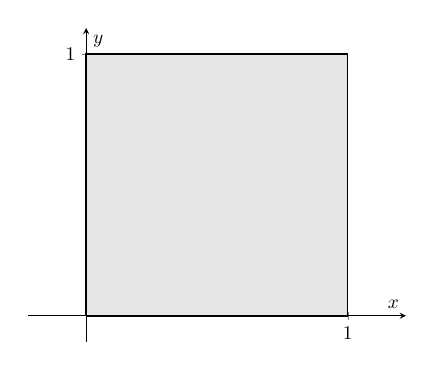
\begin{tikzpicture}[scale=0.7]
 			\begin{axis}[
 				axis lines = middle,
 				xmin = -0.1, xmax = 1.1,
 				ymin = -0.1, ymax = 1.1,
 				xtick = {0,1},
 				ytick = {0,1},
 				xlabel = $x$,
 				ylabel = $y$,
 				axis equal,
 				]
 				\addplot[
 				fill=gray!20,
 				draw=black,
 				thick
 				] coordinates {
 					(0,0) (1,0) (1,1) (0,1) (0,0)
 				};
 			\end{axis}
 		\end{tikzpicture}
 	\end{minipage}
 	\hfill
 	\begin{minipage}{0.1\textwidth}
 		\centering
 		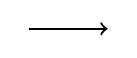
\begin{tikzpicture}
 			\draw[->, thick] (0,0) -- (1,0);
 		\end{tikzpicture}
 	\end{minipage}
 	\hfill
 	\begin{minipage}{0.55\textwidth}
 		\centering
 		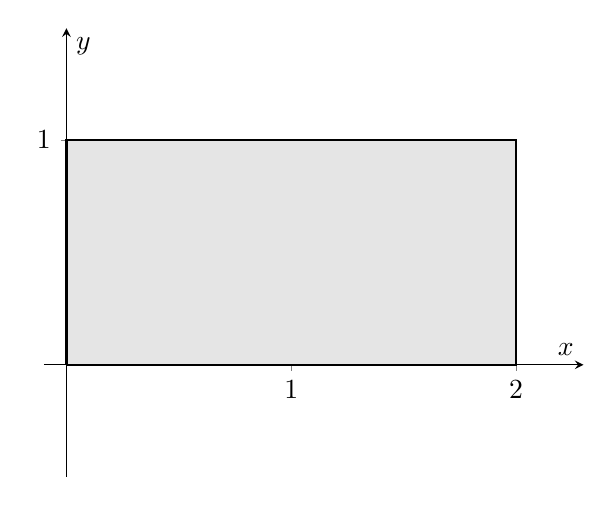
\begin{tikzpicture}[scale=1]
 			\begin{axis}[
 				axis lines = middle,
 				xmin = -0.1, xmax = 2.3,
 				ymin = -0.1, ymax = 1.1,
 				xtick = {0,1,2},
 				ytick = {0,1},
 				xlabel = $x$,
 				ylabel = $y$,
 				axis equal,
 				]
 				\addplot[
 				fill=gray!20,
 				draw=black,
 				thick
 				] coordinates {
 					(0,0) (2,0) (2,1) (0,1) (0,0)
 				};
 			\end{axis}
 		\end{tikzpicture}
 	\end{minipage}
 \end{figure}
 
 Since the area has doubled,
 
 \[
 \det(A) = 2
 \]
 
 Now, consider the matrix \(A=\begin{pmatrix}
 	-2 & 0 \\
 	0 & 1
 \end{pmatrix}\)
 
 \begin{figure}[h]
 	\centering
 	\begin{minipage}{0.3\textwidth}
 		\centering
 		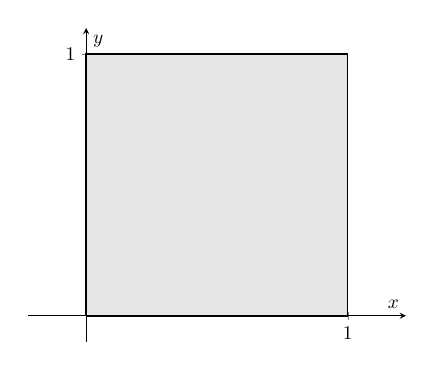
\begin{tikzpicture}[scale=0.7]
 			\begin{axis}[
 				axis lines = middle,
 				xmin = -0.1, xmax = 1.1,
 				ymin = -0.1, ymax = 1.1,
 				xtick = {0,1},
 				ytick = {0,1},
 				xlabel = $x$,
 				ylabel = $y$,
 				axis equal,
 				]
 				\addplot[
 				fill=gray!20,
 				draw=black,
 				thick
 				] coordinates {
 					(0,0) (1,0) (1,1) (0,1) (0,0)
 				};
 			\end{axis}
 		\end{tikzpicture}
 	\end{minipage}
 	\hfill
 	\begin{minipage}{0.1\textwidth}
 		\centering
 		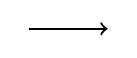
\begin{tikzpicture}
 			\draw[->, thick] (0,0) -- (1,0);
 		\end{tikzpicture}
 	\end{minipage}
 	\hfill
 	\begin{minipage}{0.55\textwidth}
 		\centering
 		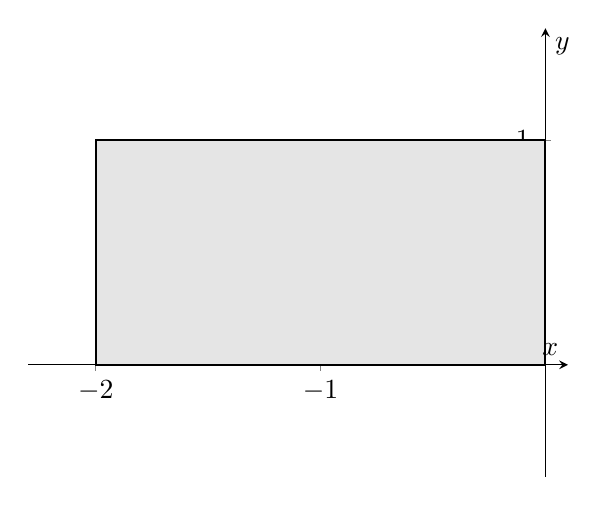
\begin{tikzpicture}[scale=1]
 			\begin{axis}[
 				axis lines = middle,
 				xmin = -2.3, xmax = 0.1,
 				ymin = -0.1, ymax = 1.1,
 				xtick = {0,-1,-2},
 				ytick = {0,1},
 				xlabel = $x$,
 				ylabel = $y$,
 				axis equal,
 				]
 				\addplot[
 				fill=gray!20,
 				draw=black,
 				thick
 				] coordinates {
 					(0,0) (-2,0) (-2,1) (0,1) (0,0)
 				};
 			\end{axis}
 		\end{tikzpicture}
 	\end{minipage}
 \end{figure}
 
 Since the volume doubled, but the orientation of the edges changed, we have
 
 
 \[
 \det(A) = -2
 \]
 
 One additional property of the determinant is
 
 \mlemma{Determinant as a Multiplicative Function}{
 If \(A, B \in M_{n\times n}(\RR)\), then
 
 \[
 \det(AB) = \det(A)\det(B)
 \]
 }
 
 \pagebreak
 
 \section{The Key Theorem of Linear Algebra}
 
 \thm{Key Theorem}{
 Let \(A \in M_{n \times n}\), then the following are equivalent:
 
 \begin{enumerate}
 	\item \(A\) is \textbf{Invertible}
 	\item \(\det(A) \neq 0\)
 	\item \(\ker(A) = 0\)
 	\item If \(\bmb\) is a column vector in \(\RR[n]\), then there is a unique column vector \(\bmx\) in \(\RR[n]\) satisfying \(A\bmx = \bmb\) 
 	\item The columns of \(A\) are linearly independent \(n \times 1\) column vectors
 	\item The rows of \(A\) are linearly independent \(n \times 1\) column vectors
 	\item \(A^t\) is invertible
 	\item All the eigenvalues of \(A\) are non-zero
 \end{enumerate}
 
 }
 
 This theorem can be expressed in terms of linear transformations,
 
 \thm{Key Theorem}{
 Let \(T: V \to V\) a linear map, then the following are equivalent:
 
 \begin{enumerate}
 	\item \(A\) is \textbf{Invertible}
 	\item \(\det(A) \neq 0\) where the determinant relies on a choice of basis on \(V\).
 	\item \(\ker(A) = 0\)
 	\item If \(b\) is a vector in \(V\), then there is a unique vector \(v \in V\) satisfying \(T(v) = b\) 
 	\item For any basis \(\{v_1, \dots,v_n\}\) of \(V\), \(T(v_1), \dots, T(v_n)\) are linearly independent.
 	\item For any basis \(\{v_1, \dots,v_n\}\) of \(V\), if \(S\) denotes the transpose linear transformation of \(T\), then \(S(v_1), \dots, S(v_n)\) are linearly independent.
 	\item The transpose of \(T\) is invertible. (Here the transpose relies on a choice of basis on \(V\))
 	\item All the eigenvalues of \(T\) are non-zero
 \end{enumerate}
 }
 
 The definitions of the determinant and transpose of a linear transformation directly depend on a choice of basis. However, the fact that \(\det(T) \neq 0\) does \textbf{not} depend on the basis chosen. Linear independence does not rely on choice of basis either.
 \pagebreak
 
 \section{Similar Matrices}
 
 When choosing a basis for an \(n\)-dimensional vector space \(V\), any linear map \(T: V \to V\) can be represented by an \(n\times n\) matrix. However, if the choice of basis changes, then the matrix representation of the same linear map will change as well.
 
 Two matrices that represent the same linear transformation under different bases will be \textbf{similar}.
 
 \dfn{Similar Matrices}{
 Two \(n \times n\) matrices \(A,B\) are \textbf{Similar} if there is an invertible matrix \(C\) such that
 
 \[
 A = C^{-1}BC
 \]
 }
 
 Given two bases for \(V\), \(\beta\) and \(\gamma\), and any \(v \in V\), we need a matrix such that
 
 \[
 C[v]_\beta=[v]_\gamma
 \]
 
 The matrix that makes this possible is
 
 \[
 C = \begin{pmatrix}
 	\mid &  & \mid \\
 	[\gamma_1]_\beta & \dots & [\gamma_n]_\beta \\
 	\mid &  & \mid
 \end{pmatrix}
 \]
 
 Then if \(T: V \to V\), \(A=[T]_\beta, \ B=[T]_\gamma\), and we have \(CA = BC\) or \(A = C^{-1}BC\), then \(A\) and \(B\) are similar.
 
 \ex{Similar Matrices}{
 Let us see the same linear map under two different bases.
 
 Let \(f: \RR[2] \to \RR[2]\) such that \(f\begin{pmatrix}
 	x \\
 	y
 \end{pmatrix} = \begin{pmatrix}
 2x \\
 x
 \end{pmatrix}\).
 
 Under the usual basis, \(E = \left\{ \colvec{1\\0}, \colvec{0\\1} \right\}\),
 
 \[
 [f]_E^E =
 \begin{pmatrix}
 	2 & 0 \\
 	1 & 0
 \end{pmatrix}
 \]
 
 Under the basis \(\beta = \left\{ \colvec{0\\1}, \colvec{1\\1} \right\}\)
 
 \[
 f\colvec{0\\1} = \colvec{0\\0}, \qquad f\colvec{1\\1} = \colvec{2\\1}
 \]
 
 \[
 \left[f\colvec{0\\1}\right]_\beta = \colvec{0\\0}, \qquad \left[f\colvec{1\\1}\right]_\beta = \left[\colvec{2\\1}\right]_\beta = \colvec{-1\\2}
 \]
 Then,
 \[
 [f]_\beta^\beta =
 \begin{pmatrix}
 	0 & -1 \\
 	0 & 2
 \end{pmatrix}
 \]
 
 Our matrix \(C\) is:
 
 \[
 E_1 = \colvec{1\\0} = -\colvec{0\\1} + \colvec{1\\1} = -\beta_1 + \beta_2, \quad \implies \quad [E_1]_\beta = \colvec{-1\\1}
 \]
 \[
 E_2 = \colvec{0\\1} = \colvec{0\\1} + 0\colvec{1\\1} = \beta_1 + 0\beta_2, \quad \implies \quad [E_2]_\beta = \colvec{1\\0}
 \]
 \[
 C = 
 \begin{pmatrix}
 	-1 & 1 \\
 	1 & 0
 \end{pmatrix}, \qquad 
 C^{-1} = 
 \begin{pmatrix}
 	0 & 1 \\
 	1 & 1
 \end{pmatrix}
 \]
 
 Such that for \(\bma \in \RR[2] \ C[\bma]_E = [\bma]_\beta\)
 
 That way, \([f]_E^E, \ [f]_\beta^\beta\) should be similar.
 
 \[
 [f]_E^E =
 \begin{pmatrix}
 	2 & 0 \\
 	1 & 0
 \end{pmatrix}
 =
 \begin{pmatrix}
 	0 & 1 \\
 	1 & 1
 \end{pmatrix}
 \begin{pmatrix}
 	0 & -1 \\
 	0 & 2
 \end{pmatrix}
 \begin{pmatrix}
 	-1 & 1 \\
 	1 & 0
 \end{pmatrix}
 =
  C^{-1}[f]_\beta^\beta C
 \]
 
 }
 
 \section{Eigenvalues and Eigenvectors}
 
 Eigenvalues and eigenvectors can be used to pick a better basis for a particular linear transformation.
 
 \dfn{Eigenvalues and Eigenvectors}{
 Let \(T: V \to V\) be a linear transformation. Then a non-zero vector \(v\) will be an \textbf{Eigenvector} of \(T\) with \textbf{Eigenvalue} \(\lambda\), a scalar, if
 
 \[T(v) = \lambda v\]
 
 For an \(n \times n\) matrix \(A\), it is the same idea, non-zero column vector \(\bmx \in \RR[n]\) eigenvector with \(\lambda\) eigenvalue if
 
 \[
 A\bmx = \lambda \bmx
 \]
 } 
 
 Geometrically, \(v\) is an eigenvector of \(T\) if \(T\) `stretches' \(v\) by a factor of \(\lambda\).
 
 \mprop{}{
 A scalar \(\lambda\) will be an \textbf{eigenvalue} of a square matrix \(A\) iff \(\lambda\) is a root of the polynomial
 
 \[
 P(t) = \det(tI-A)
 \]
 }
 
 The polynomial \(P(t)\) is called the \textbf{Characteristic Polynomial}.
 
 \thm{}{
 Let \(A,B\) be similar matrices, then their characteristic polynomial is the same.
 }
 
 \cor{}{
 The Eigenvalues for similar matrices are equal.
 }
 
 However, this does \textbf{not} imply matrices with the same eigenvalues are similar.
 
 \thm{}{
 Let \(\nlist{n}{\lambda}\) be the eigenvalues, counted with multiplicity, of a matrix \(A\). Then
 
 \[
 \det(A) = \lambda_1 \dots \lambda_n
 \]
 }
 
 Counting with multiplicity implies counting roots like \(2\) in \(P(x) = (x-2)^3\) three times.
 
 How good a basis is for a transformation depends on how close it is to being diagonal. This is far from being always possible though, but there are techniques that make is slightly better like the Jordan Normal Form.
 
 These all involve finding eigenvalues, their eigenvectors, or their generalized form.
 
 \pagebreak
 \section{Exercises}
 
 \qs{}{
 Let \(L: V \to W\) be a linear map between two vector spaces. Show that
 
 \[
 \dim(\ker(L)) + \dim(\text{Im}(L)) = \dim(V)
 \]
 } 
 
 \sol{
 Let \(\{v_1, \dots, v_m\}\) be a basis for \(\ker(L)\), with \(\dim(V) = n\). This basis may not be sufficient to span \(V\), so we add linearly independent vectors until it is a basis of \(V\).
 
 Then, \(\{v_1, \dots, v_m, v_{m+1}, \dots, v_n\}\) is a basis for \(V\).
 
 We will show \(\{L(v_{m+1}), \dots, L(v_n)\}\) is a basis for \(\text{Im}(L)\).
 
 Let \(v\in V\), we know that 
 
 \[
 v = a_1v_1 + \dots + a_mv_m + a_{m+1}v_{m+1} + \dots + a_nv_n
 \]
 
 Then,
 
 \begin{align*}
 	L(v) &= L(a_1v_1 + \dots + a_mv_m + a_{m+1}v_{m+1} + \dots + a_nv_n) \\
 	&= a_1L(v_1) + \dots + a_mL(v_m) + a_{m+1}L(v_{m+1}) + \dots + a_nL(v_n) \\
 	&= 0 + \dots + 0 + a_{m+1}L(v_{m+1}) + \dots + a_nL(v_n)
 \end{align*}
 
 \(L(v_i)\) is zero if \(i = 1, \dots, m\), because those are in \(\ker(L)\). Then, any element in \(\text{Im}(L)\) is a linear combination of \(L(v_{m+1}), \dots, L(v_n)\)
 
 Suppose there are \(a_{m+1}, \dots a_n\) such that
 
 \[
 a_{m+1}L(v_{m+1}) + \dots + a_nL(v_n) = 0
 \]
 
 Then,
 
 \[
 L(a_{m+1}v_{m+1} + \dots + a_nv_n) = 0 \quad \implies \quad a_{m+1}v_{m+1} + \dots + a_nv_n \in \ker(L)
 \]
 
 Since \(\{v_1, \dots, v_m\}\) spans \(\ker(L)\), there are \(b_1, \dots, b_m\) such that
 
 \begin{align*}
 	a_{m+1}v_{m+1} + \dots + a_nv_n &= b_1v_1 + \dots + b_nv_m \\
 	- b_1v_1 - \dots - b_mv_m + a_{m+1}v_{m+1} + \dots + a_nv_n &= 0
 \end{align*}
 
 Now, since \(\{v_1, \dots, v_m, v_{m+1}, \dots, v_n\}\) is a basis for \(V\) (then linearly independent), and this linear combination equals to zero, the \(b_j\)s and, in particular, the \(a_i\)s should all be zero. This implies that \(L(v_{m+1}), \dots, L(v_n)\) are all linearly independent, and they span \(\img(L)\); hence, they are a basis of \(\img(L)\).
 
 Calculating the dimension,
 
 \[
 \dim(\ker(L)) + \dim(\img(L)) = m + n - m = n = \dim(V)
 \]
 
 \Qed
 }
 
 \qs{}{
 Consider the set of all polynomials in one variable with real coefficients with degree less or equal to \(3\). 
 \begin{enumerate}[(a)]
 	\item Show that this set forms a vector space of dimension four.
 	\item Find a basis for this vector space.
 	\item Show that differentiating a polynomial is a linear map.
 	\item Given the basis in (b), write down the matrix representative of the derivative.
 \end{enumerate}
 }
 \sol{
 \begin{enumerate}[(a)]
 	\item Let \(P_3 = \{ a_0 + a_1x + a_2x^2 + a_3x^3 \mid a_i \in \RR\}\). Manually checking the conditions for a vector space here works. 
 	
 	The set \(\{1, x, x^2, x^3\}\) is a linearly independent set since 
 	 \[
 	 a_0 + a_1x + a_2x^2 + a_3x^3 = 0
 	 \]
 	 does imply \(a_i = 0 \ \forall i\).
 	 
 	 The set also evidently spans \(P_3\) since all polynomials are already a linear combination of these elements.
 	 
 	 Since the basis has four elements, \(\dim(P_3) = 4\).
 	 
 	 \item \(\{1, x, x^2, x^3\}\).
 	 \item Let's consider the map \(\frac{d}{dx} : P_3 \to P_2\) defined by
 	 
 	 \[
 	 \frac{d}{dx}(a_0 + a_1x + a_2x^2 + a_3x^3) = a_1 + 2a_2x + 3a_3x^2 
 	 \]
 	 
 	 Given two polynomials in \(P_3\), \(a_0 + a_1x + a_2x^2 + a_3x^3\) and \(b_0 + b_1x + b_2x^2 + b_3x^3\)
 	 
 	 \begin{align*}
 	 	&\phantom{=} \frac{d}{dx}\left( \lambda_1(a_0 + a_1x + a_2x^2 + a_3x^3) + \lambda_2(b_0 + b_1x + b_2x^2 + b_3x^3)\right) \\
 	 	&= \frac{d}{dx}\left( (\lambda_1a_0 + \lambda_2 b_0) + (\lambda_1a_1 + \lambda_2b_1)x + (\lambda_1a_2 + \lambda_2b_2)x^2 + (\lambda_1a_3 + \lambda_2b_3)x^3\right) \\
 	 	&= (\lambda_1a_1 + \lambda_2b_1) + 2(\lambda_1a_2 + \lambda_2b_2)x + 3(\lambda_1a_3 + \lambda_2b_3)x^2 \\
 	 	&= \lambda_1(a_1 + 2a_2x + 3a_3 x^2) +  \lambda_2(b_1 + 2b_2x + 3b_3 x^2)\\
 	 	&=  \lambda_1\frac{d}{dx}(a_0 + a_1x + a_2x^2 + a_3x^3) + \lambda_2\frac{d}{dx}(b_0 + b_1x + b_2x^2 + b_3x^3)
 	 \end{align*}
 	 And \(\frac{d}{dx}\) is linear.
 	 \Qed
 	 
 	 \item Given the bases \(\beta = \{1, x, x^2, x^3\}\) and \(\gamma = \{1, x, x^2\}\) for \(P_3\) and \(P_2\),
 	 
 	 \[
 	 \frac{d}{dx}(1) = 0, \quad
 	 \frac{d}{dx}(x) = 1, \quad
 	 \frac{d}{dx}(x^2) = 2x, \quad
 	 \frac{d}{dx}(x^3) = 3x^2, \quad
 	 \]
 	 
 	 When translating to the basis \(\gamma\),
 	 
 	 \[
 	 \left[\frac{d}{dx}(1)\right]_\gamma = \colvec{0\\0\\0}, \quad
 	 \left[\frac{d}{dx}(x)\right]_\gamma = \colvec{1\\0\\0}, \quad
 	 \left[\frac{d}{dx}(x^2)\right]_\gamma = \colvec{0\\2\\0}, \quad
 	 \left[\frac{d}{dx}(x^3)\right]_\gamma = \colvec{0\\0\\3}, \quad
 	 \]
 	 
 	 So the matrix representation of \(\frac{d}{dx}\) is:
 	 
 	 \[
 	 \left[\frac{d}{dx}\right]_\beta^\gamma = 
 	 \begin{pmatrix}
 	 	0 & 1 & 0 & 0 \\
 	 	0 & 0 & 2 & 0 \\
 	 	0 & 0 & 0 & 3
 	 \end{pmatrix}
 	 \]
 	 
 	 Using it on \(p(x) = 3 + 7x + 5x^3\) for example,
 	 
 	 \[
 	 \begin{pmatrix}
 	 	0 & 1 & 0 & 0 \\
 	 	0 & 0 & 2 & 0 \\
 	 	0 & 0 & 0 & 3
 	 \end{pmatrix}
 	 \colvec{3\\7\\0\\5}
 	 =
 	 \colvec{7\\0\\15}
 	 \]
 	 
 	 Which corresponds to \(7 + 15x^2\).
 	 
 \end{enumerate}
 }
 I had never seen this way of portraying the derivative as a matrix. This must be the way computers do derivatives, unless there is an even more efficient way to do them, matrix multiplication is very costly.
 
\end{document}
